% Copyright 2004 by Till Tantau <tantau@users.sourceforge.net>.
%
% In principle, this file can be redistributed and/or modified under
% the terms of the GNU Public License, version 2.
%
% However, this file is supposed to be a template to be modified
% for your own needs. For this reason, if you use this file as a
% template and not specifically distribute it as part of a another
% package/program, I grant the extra permission to freely copy and
% modify this file as you see fit and even to delete this copyright
% notice. 

\documentclass{beamer}
\graphicspath{{plot/}}

% There are many different themes available for Beamer. A comprehensive
% list with examples is given here:
% http://deic.uab.es/~iblanes/beamer_gallery/index_by_theme.html
% You can uncomment the themes below if you would like to use a different
% one:
%\usetheme{AnnArbor}
%\usetheme{Antibes}
%\usetheme{Bergen}
%\usetheme{Berkeley}
%\usetheme{Berlin}
%\usetheme{Boadilla}
%\usetheme{boxes}
%\usetheme{CambridgeUS}
%\usetheme{Copenhagen}
%\usetheme{Darmstadt}
%\usetheme{default}
%\usetheme{Frankfurt}
%\usetheme{Goettingen}
%\usetheme{Hannover}
%\usetheme{Ilmenau}
%\usetheme{JuanLesPins}
%\usetheme{Luebeck}
\usetheme{Madrid}
%\usetheme{Malmoe}
%\usetheme{Marburg}
%\usetheme{Montpellier}
%\usetheme{PaloAlto}
%\usetheme{Pittsburgh}
%\usetheme{Rochester}
%\usetheme{Singapore}
%\usetheme{Szeged}
%\usetheme{Warsaw}

\title{Analysis of Human Performance in Stress Activities}

% A subtitle is optional and this may be deleted

\author{Suchismitha\inst{1} \and Lavanya\inst{2}\and Yashwanth\inst{3}}
% - Give the names in the same order as the appear in the paper.
% - Use the \inst{?} command only if the authors have different
%   affiliation.


\date{May 4, 2018}
% - Either use conference name or its abbreviation.
% - Not really informative to the audience, more for people (including
%   yourself) who are reading the slides online

% This is only inserted into the PDF information catalog. Can be left
% out. 

% If you have a file called "university-logo-filename.xxx", where xxx
% is a graphic format that can be processed by latex or pdflatex,
% resp., then you can add a logo as follows:

% \pgfdeclareimage[height=0.5cm]{university-logo}{university-logo-filename}
% \logo{\pgfuseimage{university-logo}}

% Delete this, if you do not want the table of contents to pop up at
% the beginning of each subsection:
%\AtBeginSubsection[]
%{
 % \begin{frame}<beamer>{Outline}
 %   \tableofcontents[currentsection,currentsubsection]
 % \end{frame}
%}

% Let's get started
\begin{document}
\begin{frame}
  \titlepage
\end{frame}

\begin{frame}{Outline}
  \tableofcontents
  % You might wish to add the option [pausesections]
\end{frame}

% Section and subsections will appear in the presentation overview
% and table of contents.
\section{Motivation}
\section{Data Cleaning and Reorganization}
\section{Initial Analysis}
\subsection{Correlation}
\section{Quality Control}
\section{Linear Model}
\section{Hypothesis Testing}
\section{Summary}


\begin{frame}{Initial Analysis}{Correlation}
  \begin{figure}
	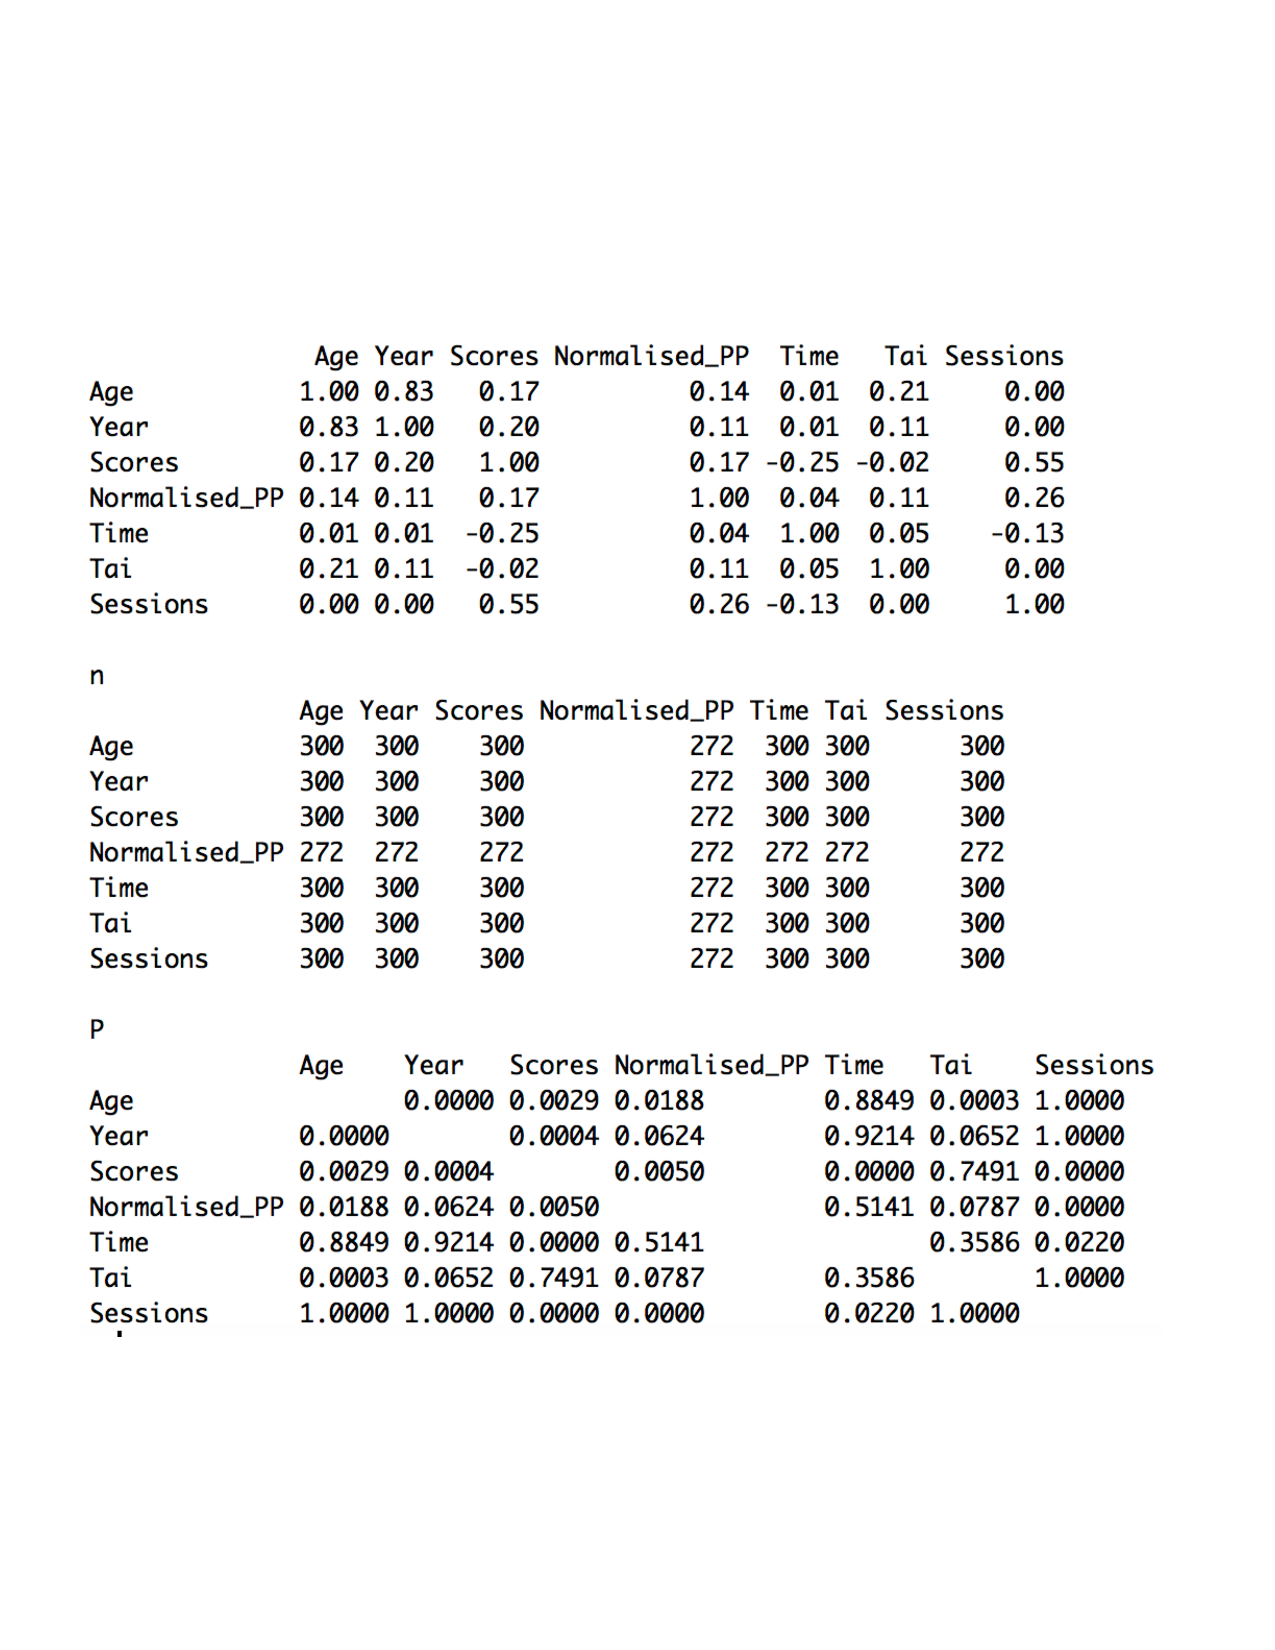
\includegraphics[width=0.6\textwidth]{Correlation_Data.pdf}
	\caption{Correlation Matrix}
\end{figure} 
\end{frame}

\begin{frame}{Quality Control}{Biographic data }

% You can reveal the parts of a slide one at a time
  \begin{itemize}
  \item {
    By referring to the Bar plot of gender distribution we can infer that the number of male subjects more than the number of female subjects 
  }
  \item {   
    Number of female subject is half as number of male subjects 
  }
    \end{itemize}
    \begin{figure}
	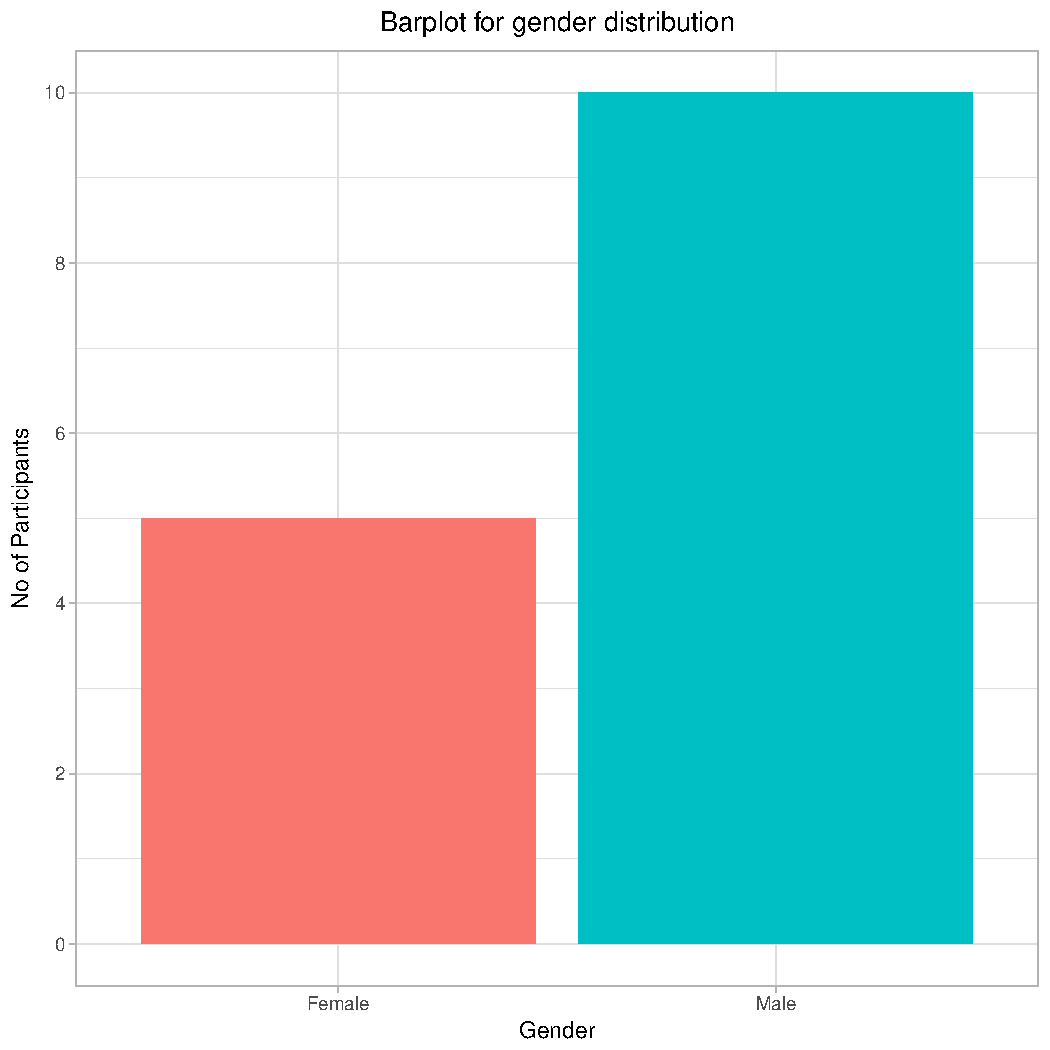
\includegraphics[width=0.4\textwidth]{1_gender.pdf}
	\caption{Gender Distribution}
\end{figure}
 \end{frame}
\begin{frame}{Quality Control}{Biographic data Contd. }

% You can reveal the parts of a slide one at a time
  \begin{itemize}
  \item {
    By referring to the Bar plot of Age distribution , we can infer that more number of subjects are in the age group 22 and 23
  }
  \item {   
   Also we can see from the dataset that few subjects age has been changed over the period of study 
  }
    \end{itemize}
    \begin{figure}
	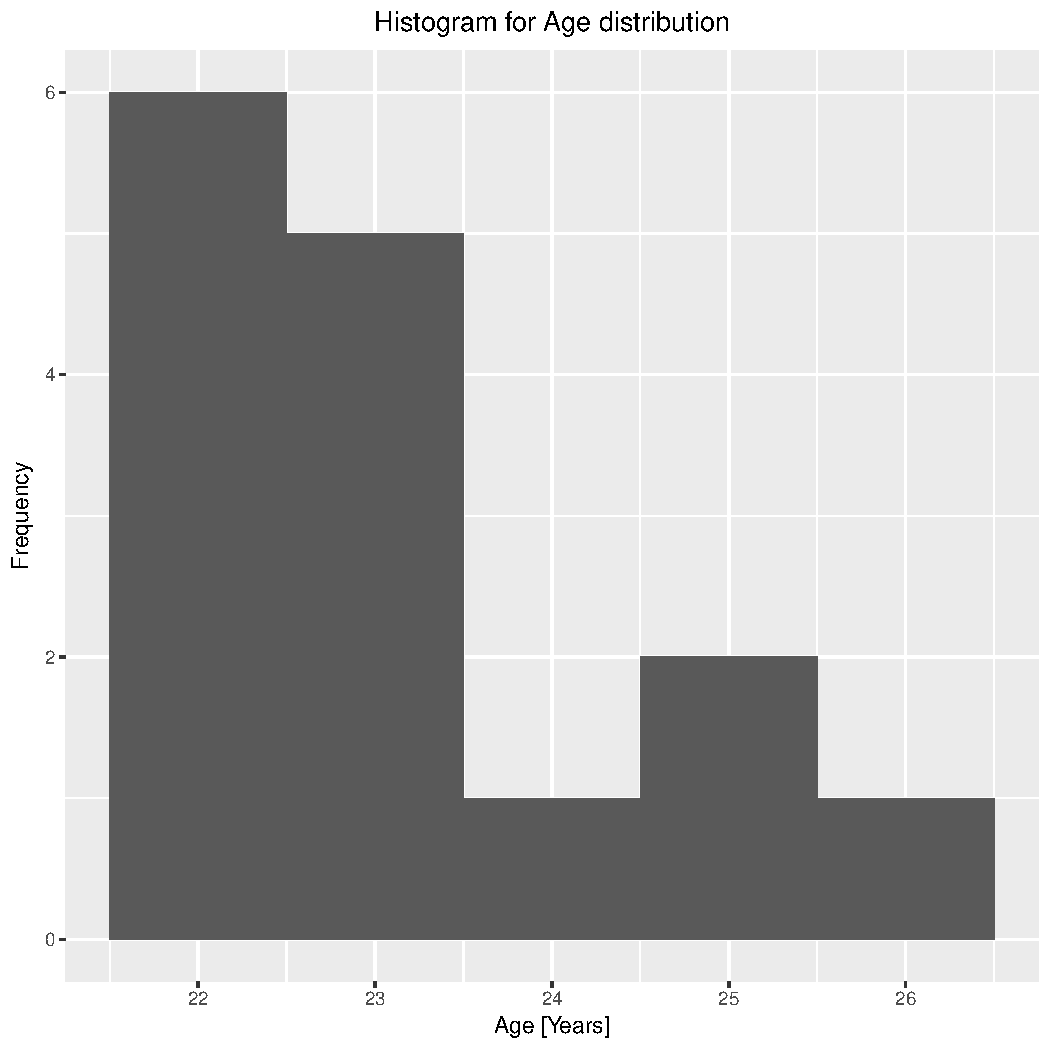
\includegraphics[width=0.4\textwidth]{1_age.pdf}
	
\end{figure}
 \end{frame}

\begin{frame}{Quality Control}{Trait Psychometric Data }

% You can reveal the parts of a slide one at a time
  \begin{itemize}
  \item {
    Trait Anxiety Inventory(TAI) scores}
\item {Range 20-80 }
\item {Higher value of Tai indicates   over anxious individuals }
\item {Most of the subjects had TAI scores in the range 25-55}
    \end{itemize}
    \begin{figure}
	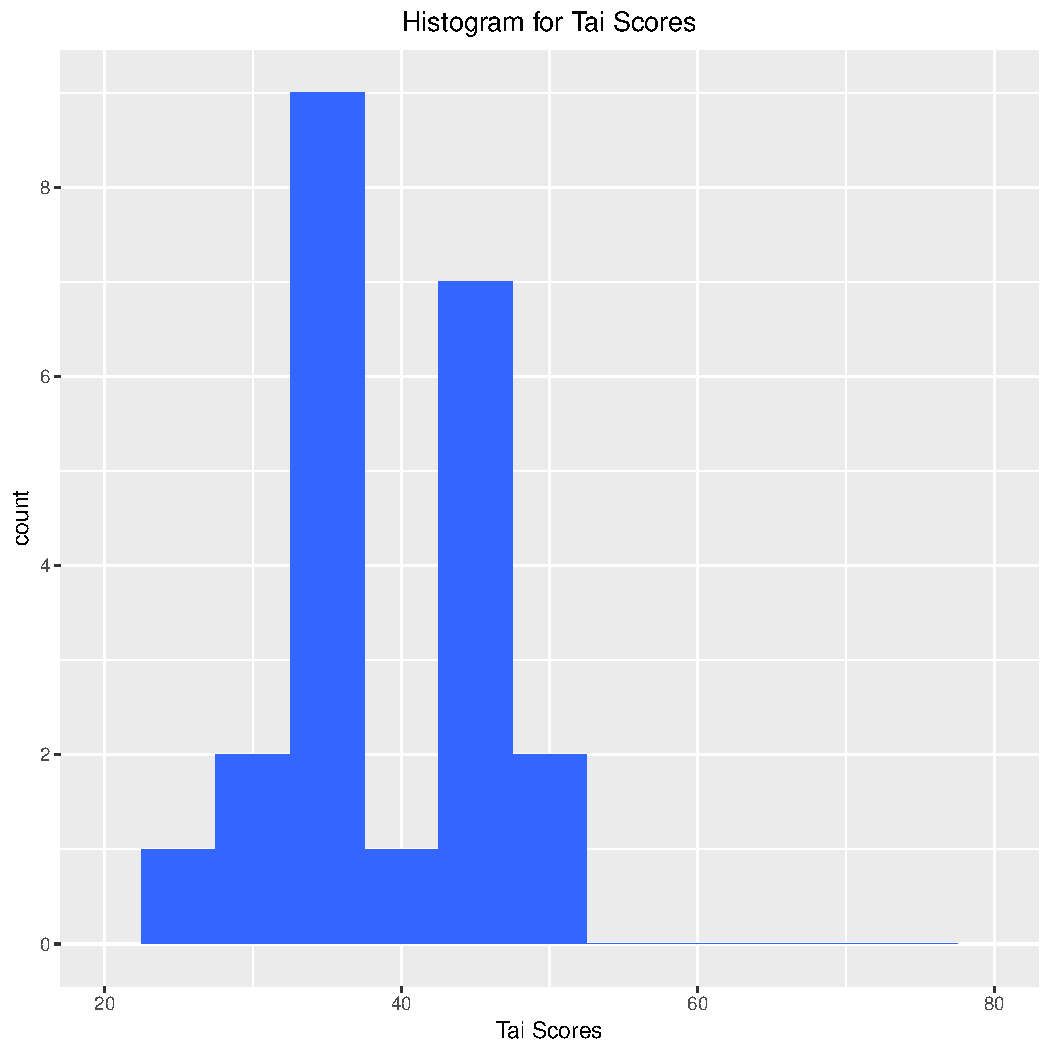
\includegraphics[width=0.4\textwidth]{tai_plot.pdf}
	
\end{figure}
 \end{frame}
\begin{frame}{Quality Control}{State Psychometric  data }

% You can reveal the parts of a slide one at a time
  \begin{itemize}
  \item {
   Downward Trend}
  \item {   As we can see from the plot the effort , frustration , mental demand , performance and physical demand , temporal demand are all maintaining a downward trend
}
      \end{itemize}
    \begin{figure}
	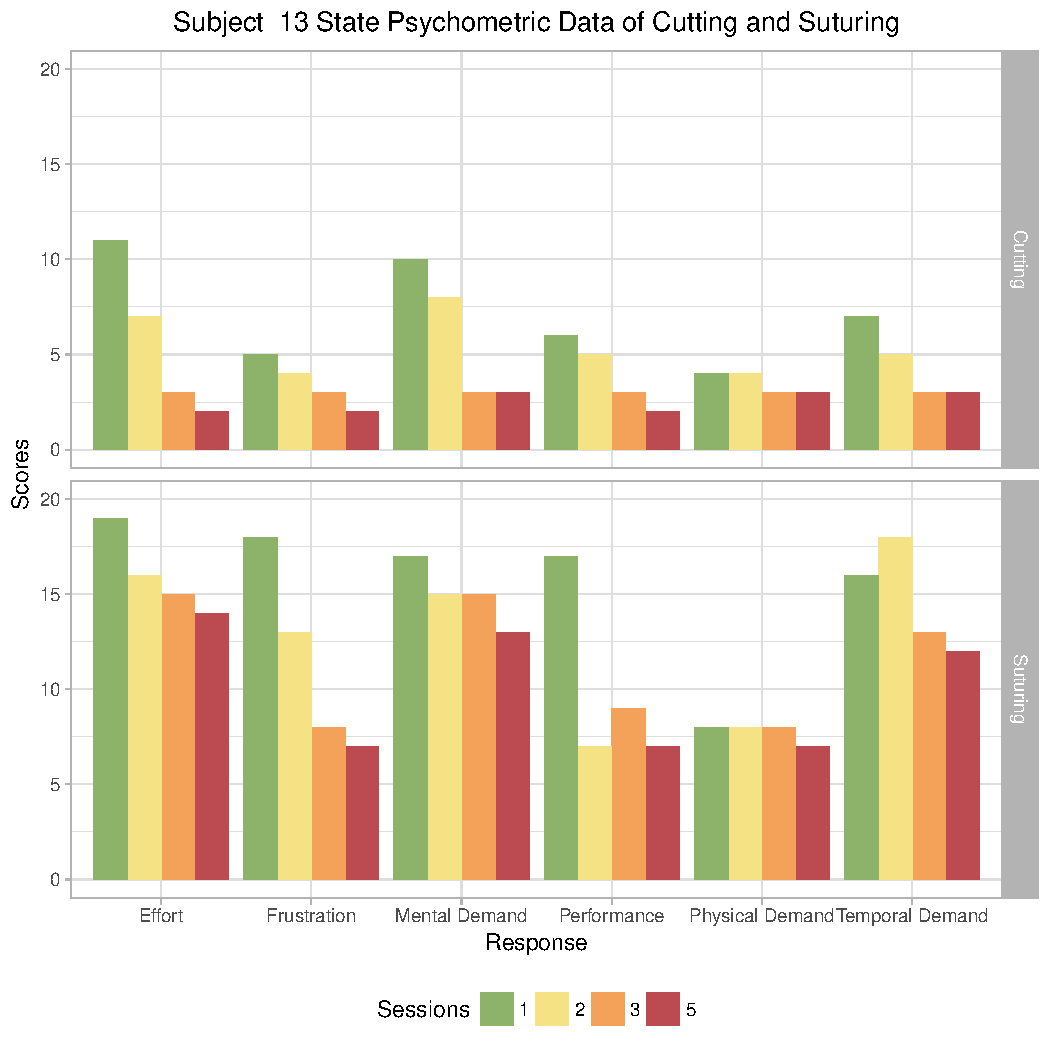
\includegraphics[width=0.45\textwidth]{subject13_State_Psychometric_Data_of_Cutting_and_Suturing.pdf}
	\end{figure}
 \end{frame}
\begin{frame}{Quality Control}{Perinasal Perspiration (Stress) Signal Data }

% You can reveal the parts of a slide one at a time
  \begin{itemize}
  \item {
   While performing Suturing Stress signals were observed for more duration }
  \item {Suturing is more strenuous task }
  \item {Baseline is at the lower level }
  \item {Down sampling of data - Averaged data will give smoother signals }
      \end{itemize}
    \begin{figure}
	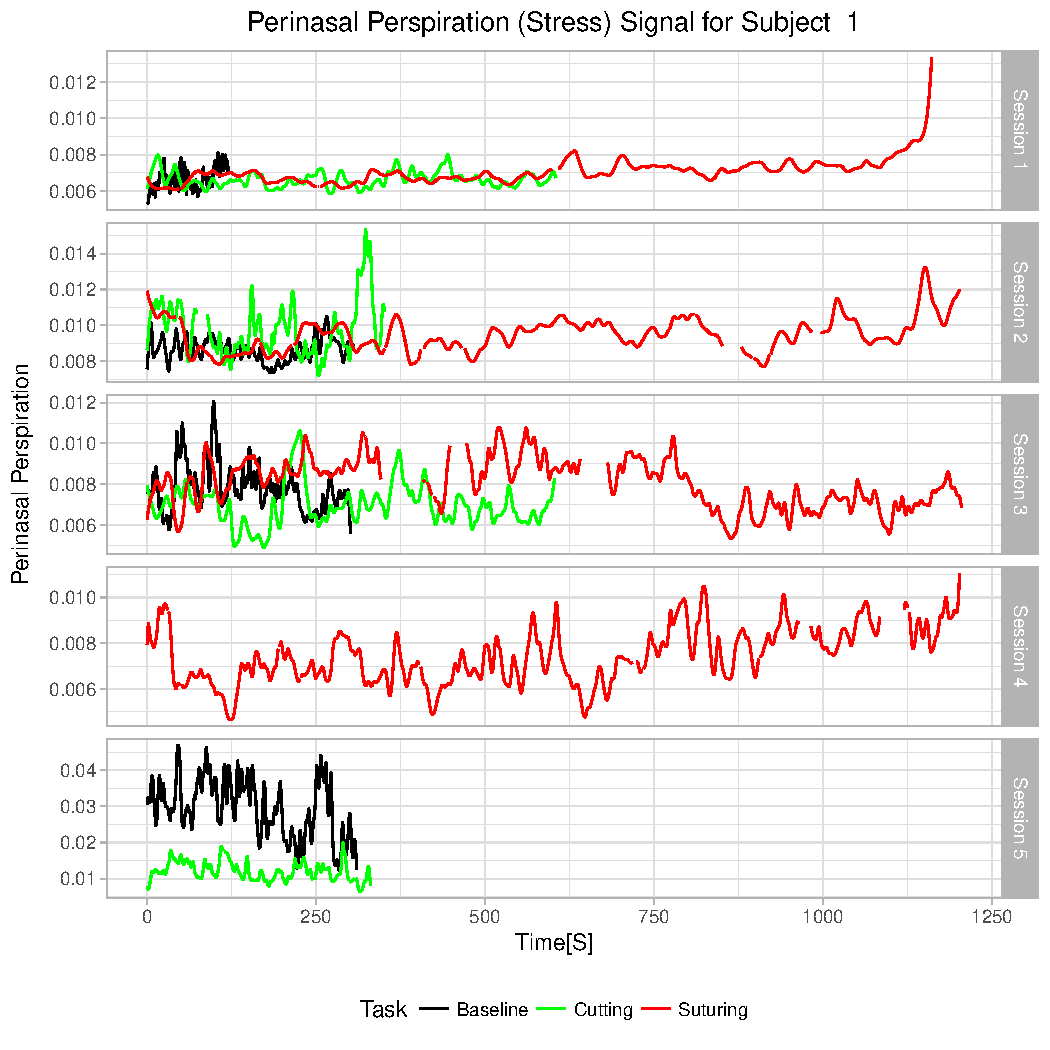
\includegraphics[width=0.4\textwidth]{01_Perinasal_Perspiration.pdf}
	\end{figure}
 \end{frame}
 
 
\begin{frame}{Quality Control}{Performance Data }

% You can reveal the parts of a slide one at a time
  \begin{itemize}
  \item {
  Time taken by subject to perform cutting is decreasing session by session and Downward trend for Cutting task }
 \item {The Subject has mastered the task of cutting and can do it faster after each session, It is not the same in case of suturing, as we have already observed from peri nasal perspiration data }
 \item {suturing is more strenuous task so It takes more time to finish}
      \end{itemize}
    \begin{figure}
	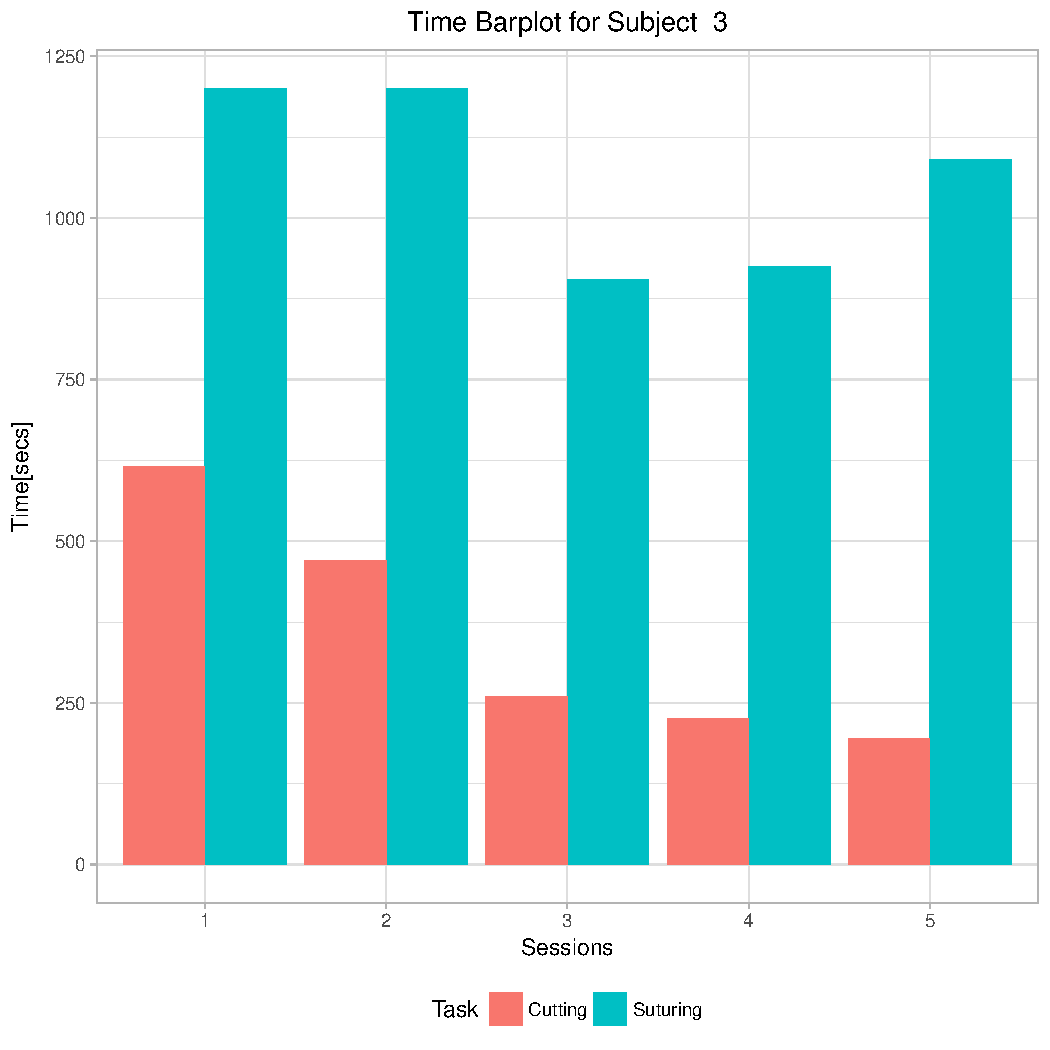
\includegraphics[width=0.35\textwidth]{3_Time_barplot.pdf}
	\end{figure}
 \end{frame}
\begin{frame}{Quality Control}{Performance Data Contd.}
\begin{itemize}
  \item {
  We can observe Ascending trend }
  \item {The scores obtained for cutting and suturing is increasing for each session}
  \item {The subject is becoming more adept in the tasks }

      \end{itemize}
    \begin{figure}
	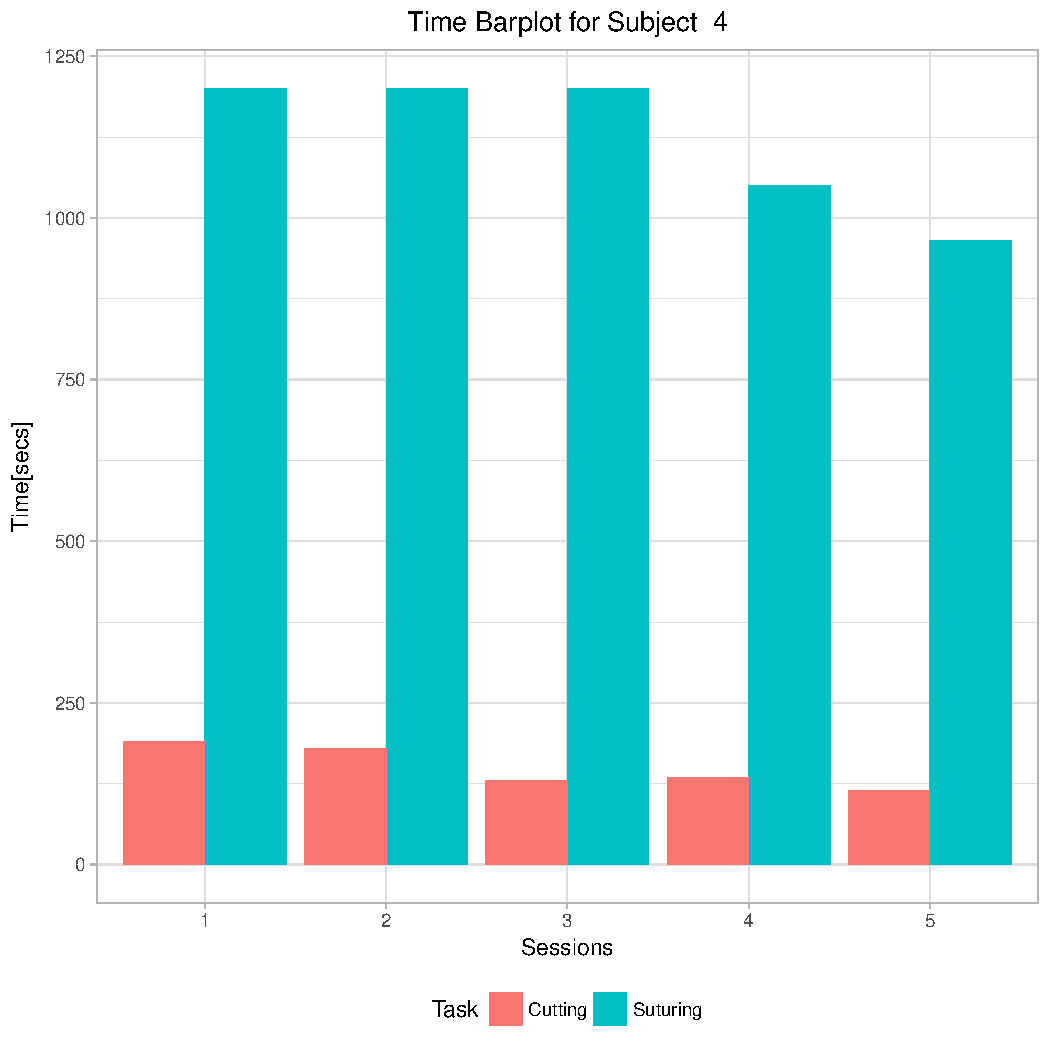
\includegraphics[width=0.45\textwidth]{4_Time_barplot.pdf}
	\end{figure}
 \end{frame}

\begin{frame}{Linear Model}{ Score with all Other attributes}
Null Hypothesis : $H_0$ =  The score obtained does not depend on the demographics of the subject , session , age , year , sex and perspiration.\\
Alternate Hypothesis : $H_1$ =  The score obtained  depends on the demographics of the subject , session , age , year , sex and perspiration.\\
\begin{figure}
	\centering
	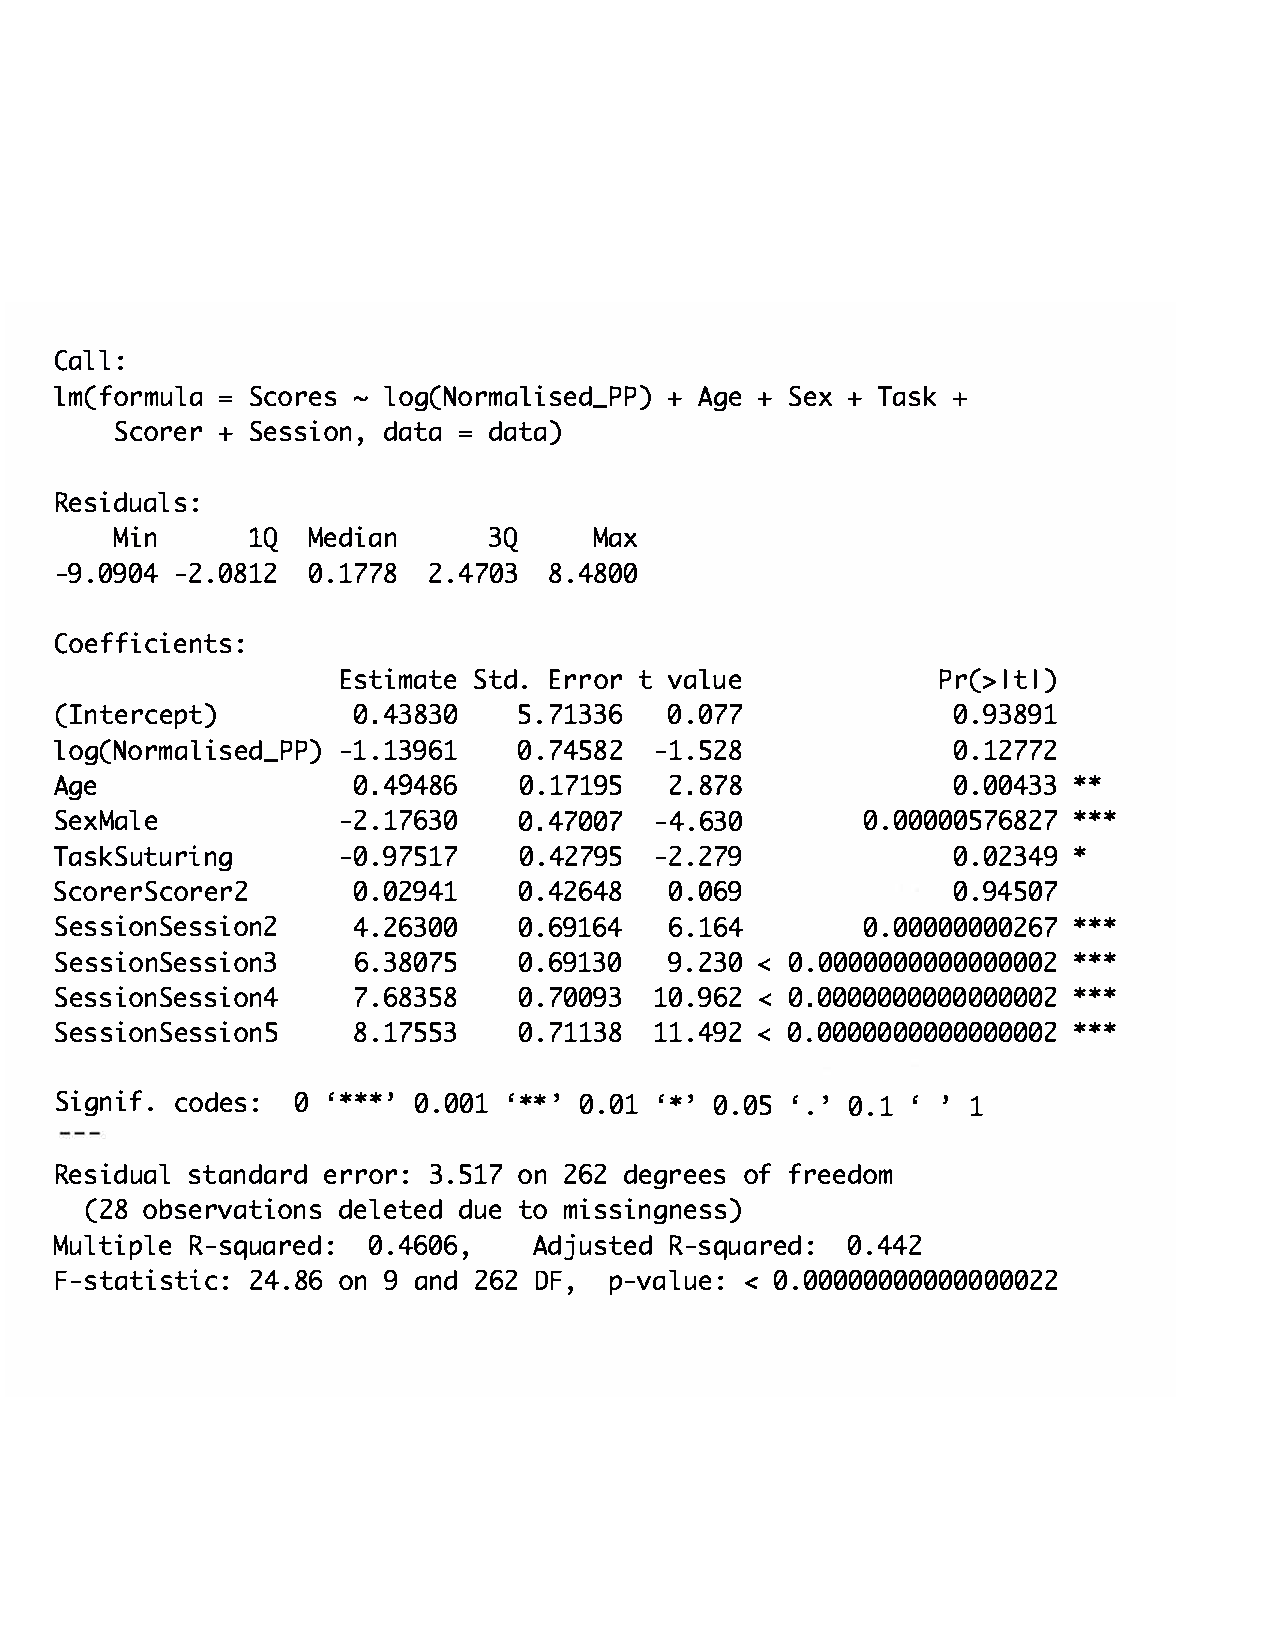
\includegraphics[width=0.5\textwidth]{ScoreSummary.pdf}
	\centering
\end{figure}
 \end{frame}
\begin{frame}{Linear Model}{ Score with all Other attributes Contd,}
\begin{figure}
	\begin{minipage}[c]{0.4\linewidth}
	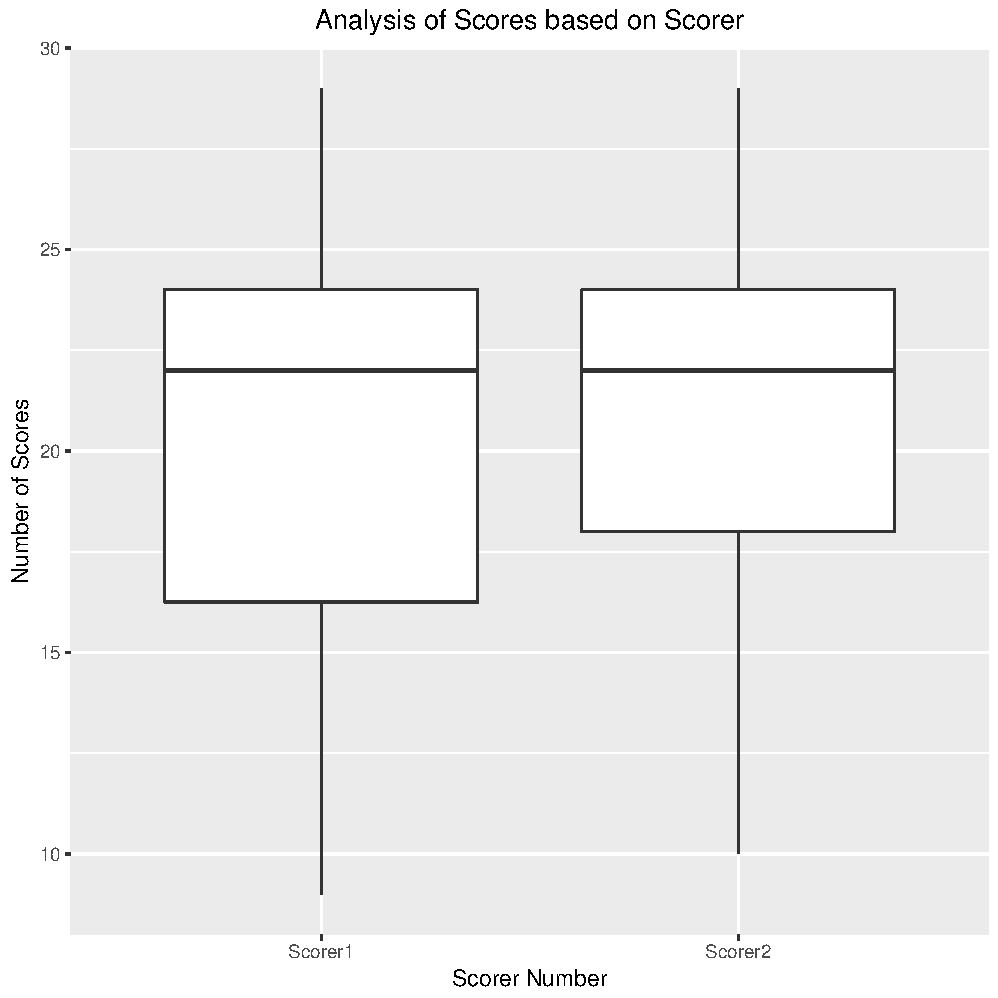
\includegraphics[width=\linewidth]{ScorerVsScore.pdf}
	\end{minipage}
	\hfill
	\begin{minipage}[c]{0.4\linewidth}
	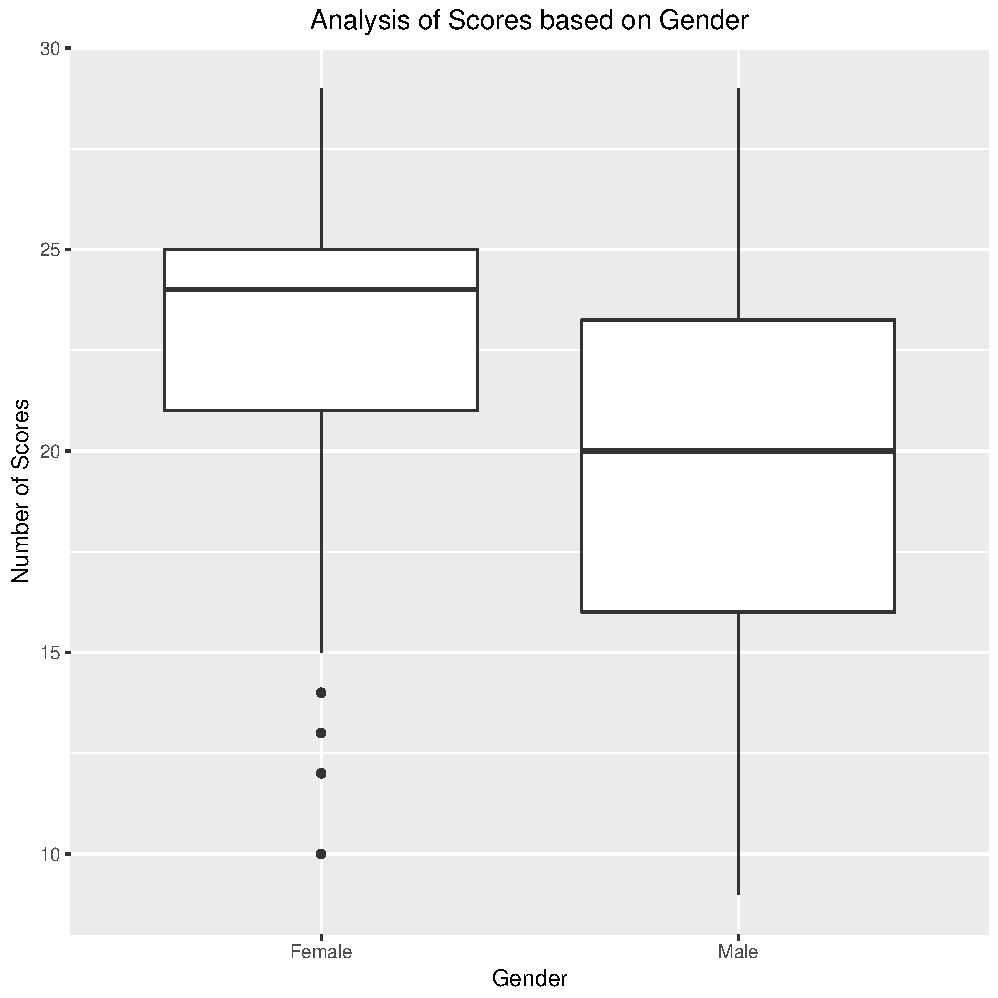
\includegraphics[width=\linewidth]{GenderVsScore.pdf}
	\end{minipage}
\end{figure}
\begin{figure}
	\begin{minipage}[c]{0.4\linewidth}
	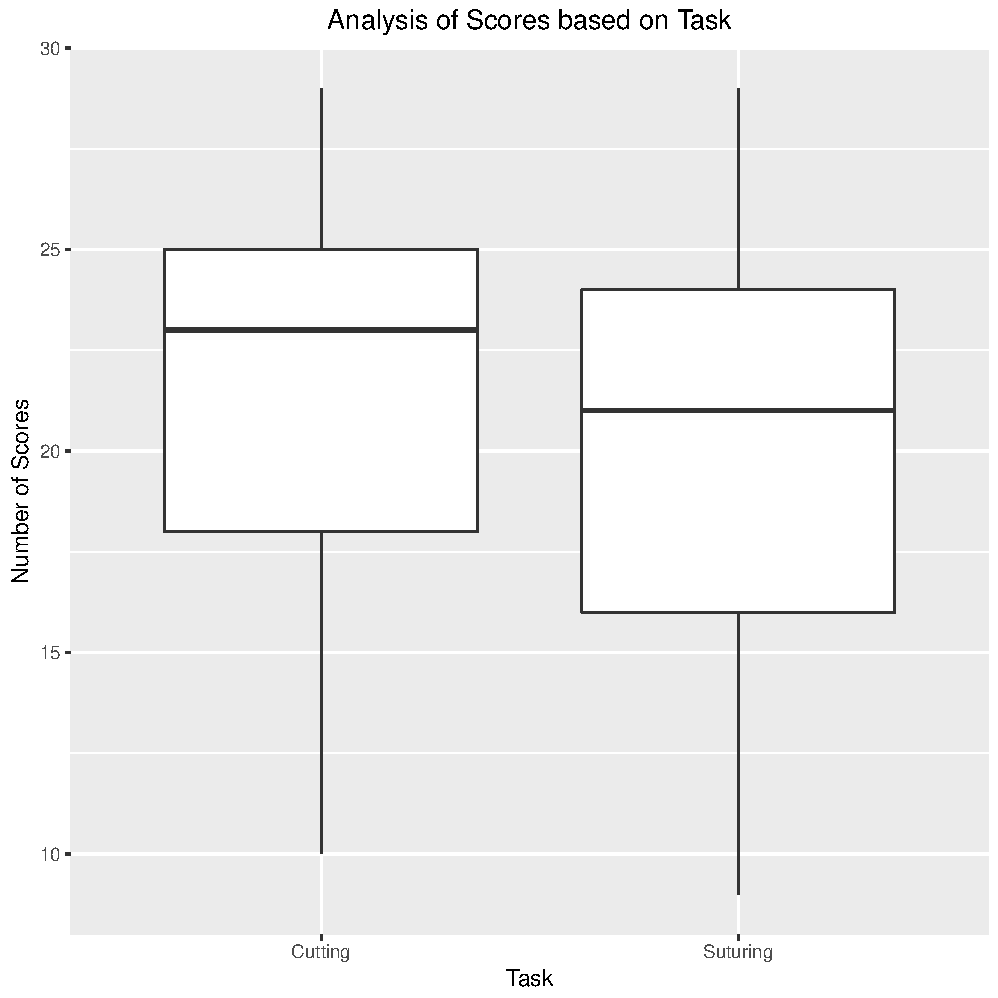
\includegraphics[width=\linewidth]{TaskVsScore.pdf}
	\end{minipage}
	\hfill
	\begin{minipage}[c]{0.4\linewidth}
	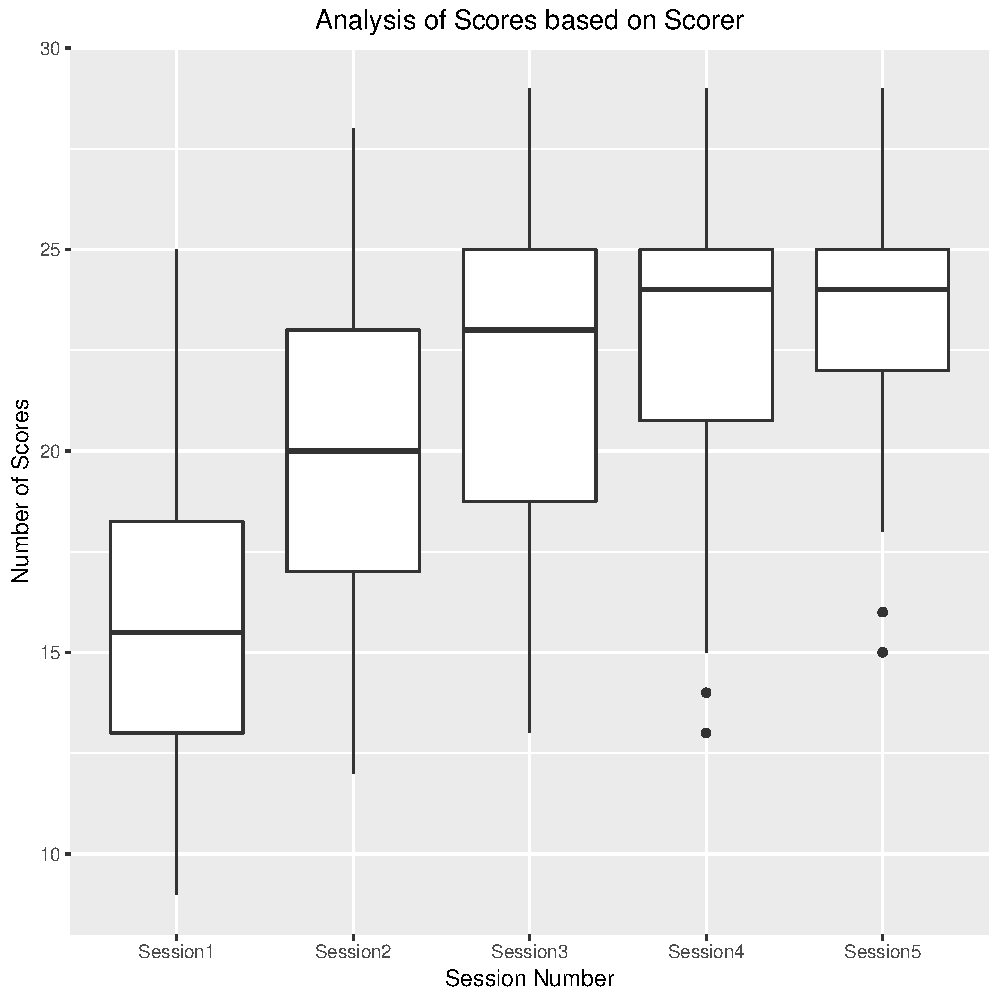
\includegraphics[width=\linewidth]{SessionVsScore.pdf}
	\end{minipage}
\end{figure}
 \end{frame}


\begin{frame}{Linear Model}{ Time with all Other attributes}
Null Hypothesis : $H_0 $=  The time taken to do a task is not dependent of age, session, sex, Perspiration.\\
Alternate Hypothesis : $H_1$ =  he time taken to do a task depends on  age, session, sex, Perspiration.
\begin{figure}
	\centering
	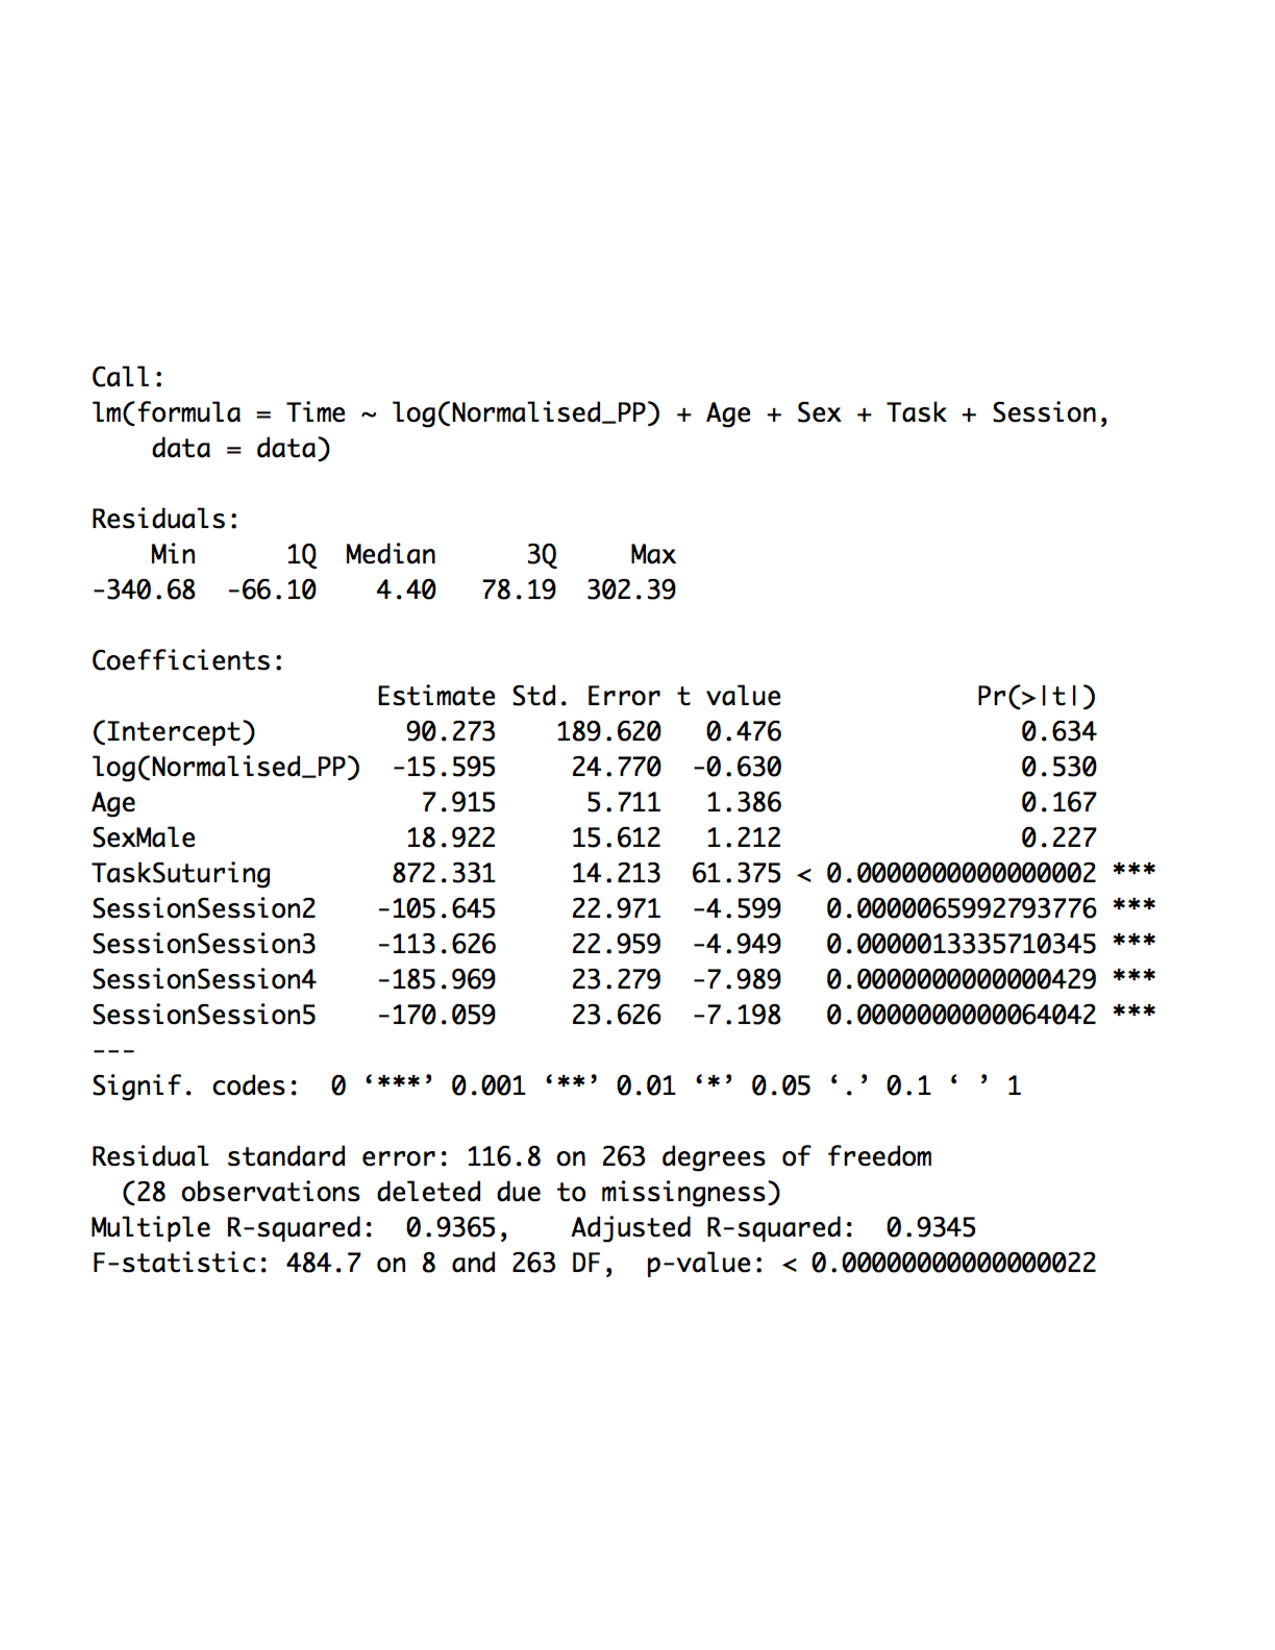
\includegraphics[width=0.5\textwidth]{TimeSummary.pdf}
	\centering
\end{figure}
 \end{frame}
\begin{frame}{Linear Model}{ Time with all Other attributes Contd,}
\begin{figure}
	\begin{minipage}[c]{0.4\linewidth}
	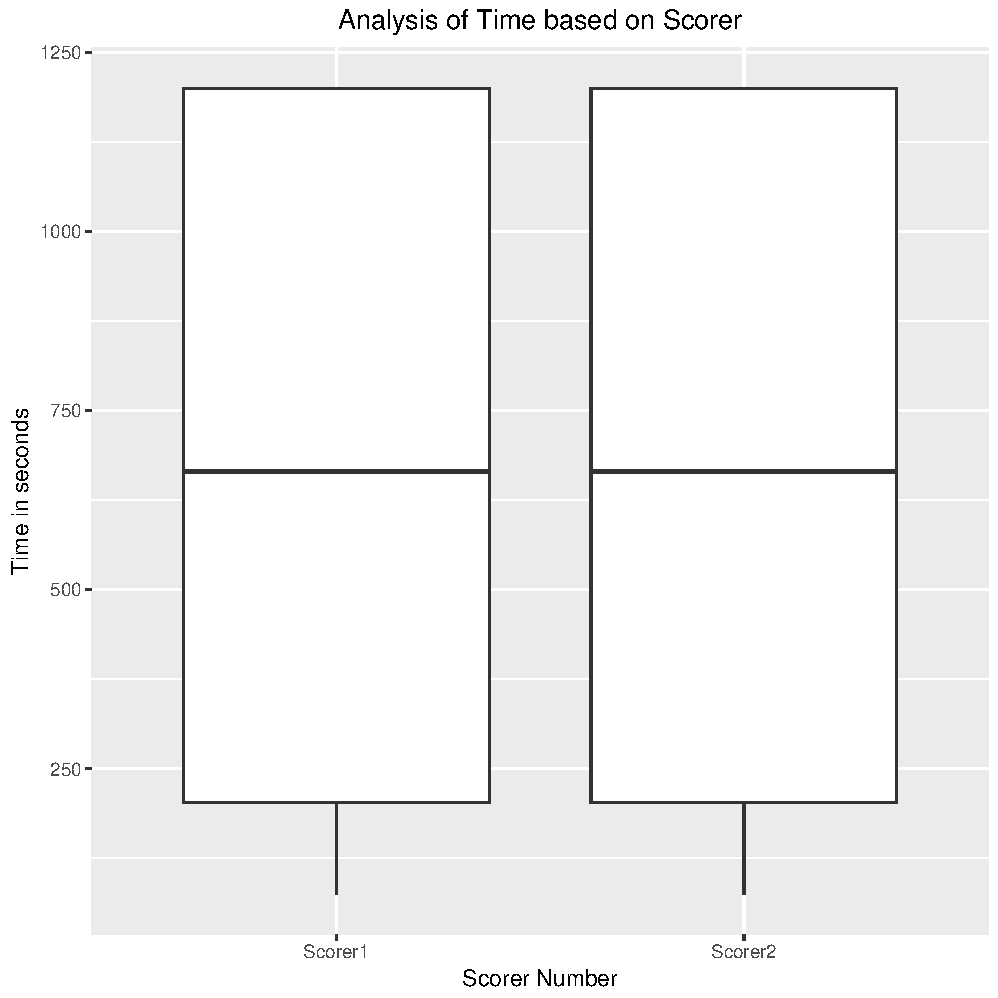
\includegraphics[width=\linewidth]{ScorerVsTime.pdf}
	\end{minipage}
	\hfill
	\begin{minipage}[c]{0.4\linewidth}
	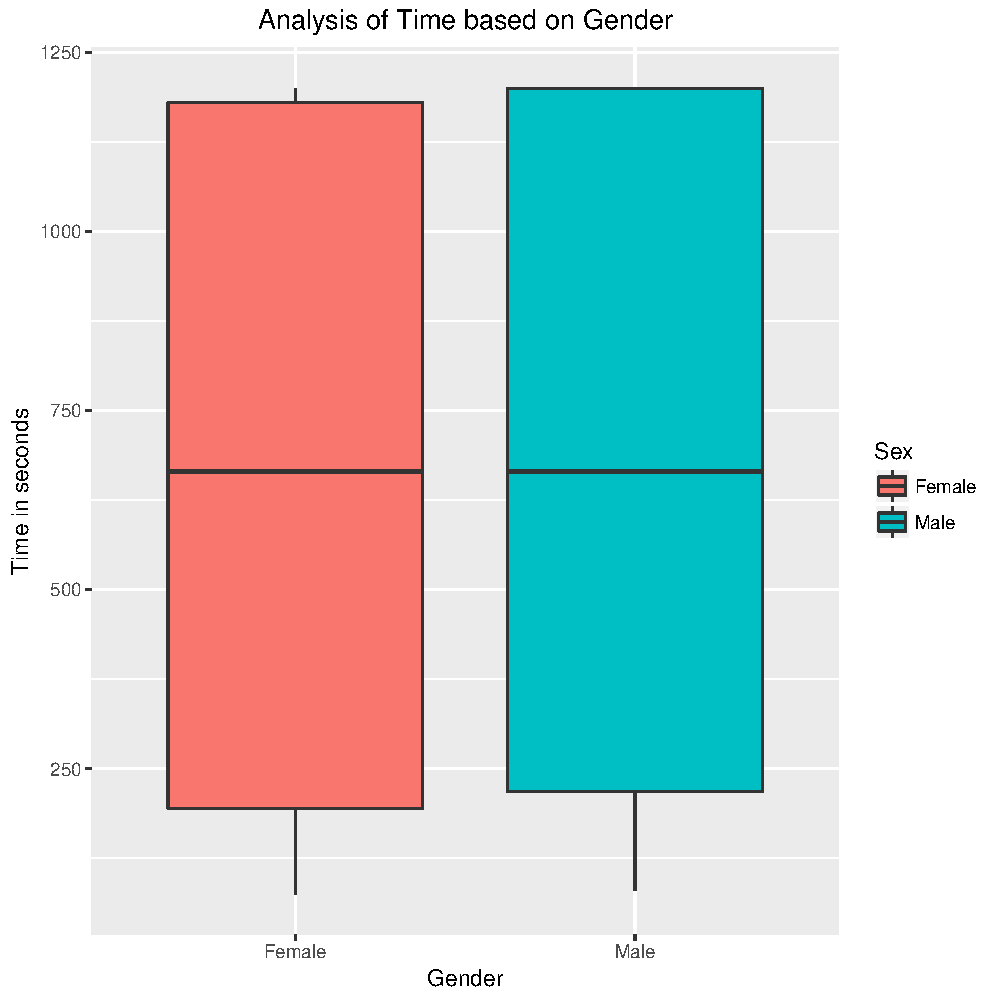
\includegraphics[width=\linewidth]{GenderVsTime.pdf}
	\end{minipage}
\end{figure}
\begin{figure}
	\begin{minipage}[c]{0.4\linewidth}
	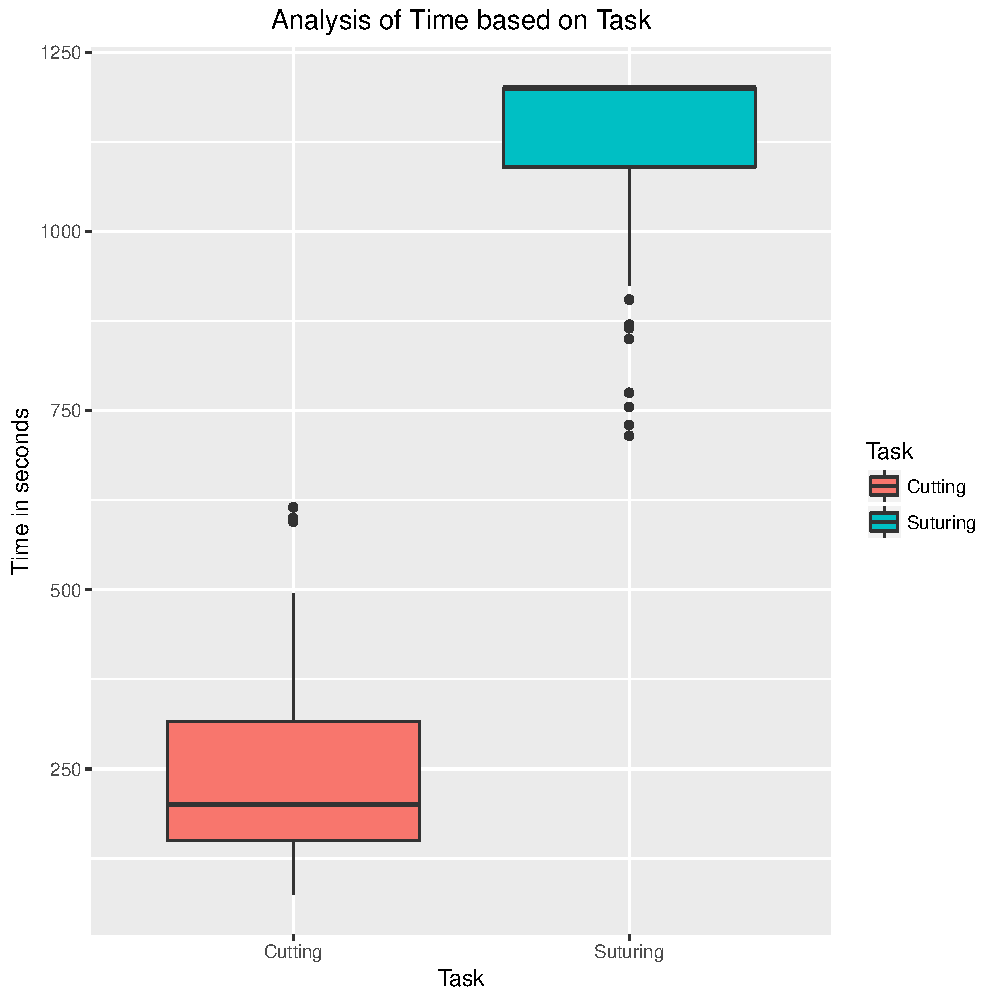
\includegraphics[width=\linewidth]{TaskVsTime.pdf}
	\end{minipage}
	\hfill
	\begin{minipage}[c]{0.4\linewidth}
	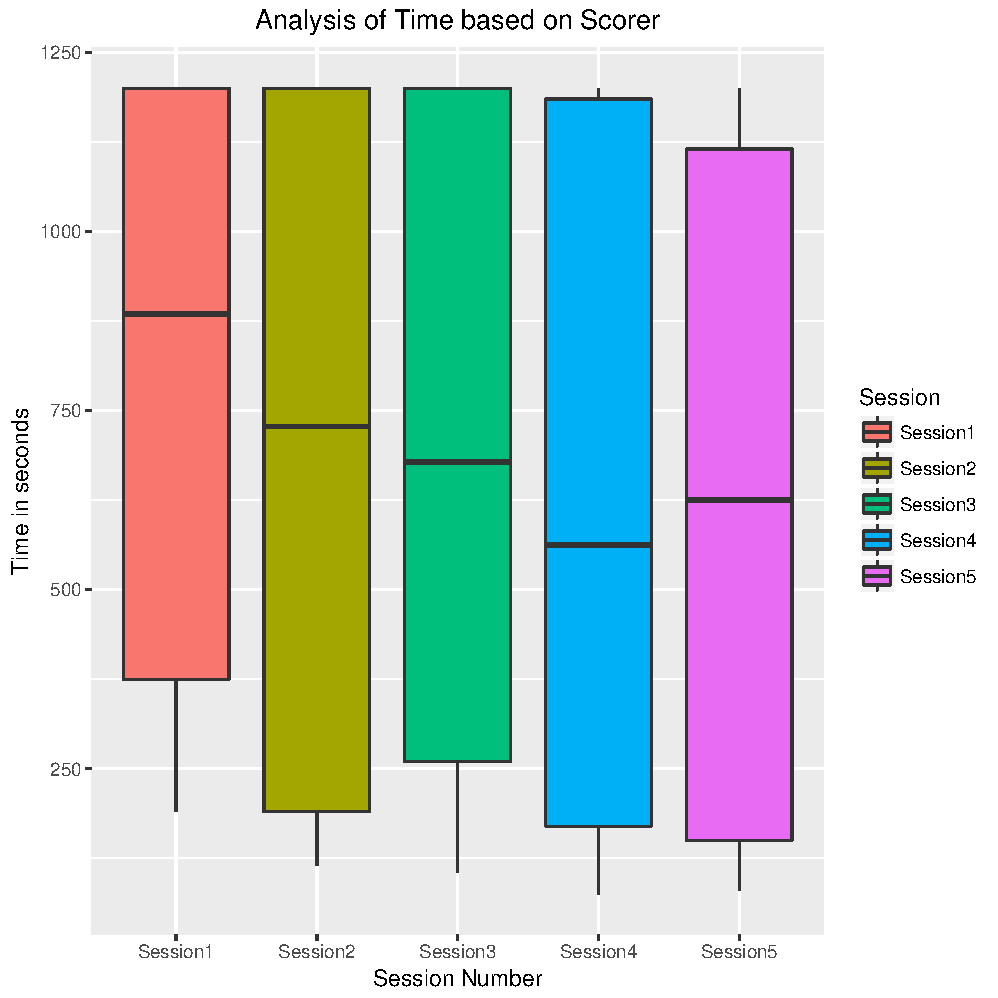
\includegraphics[width=\linewidth]{SessionVsTime.pdf}
	\end{minipage}
\end{figure}
 \end{frame}
 
\begin{frame}{Linear Model}{ Performance Analysis of Suturing Task}
\begin{itemize}
  \item {The number of sutures increases with each session.}
      \end{itemize}
\begin{figure}[!htb]
	\begin{minipage}[c]{0.45\linewidth}
	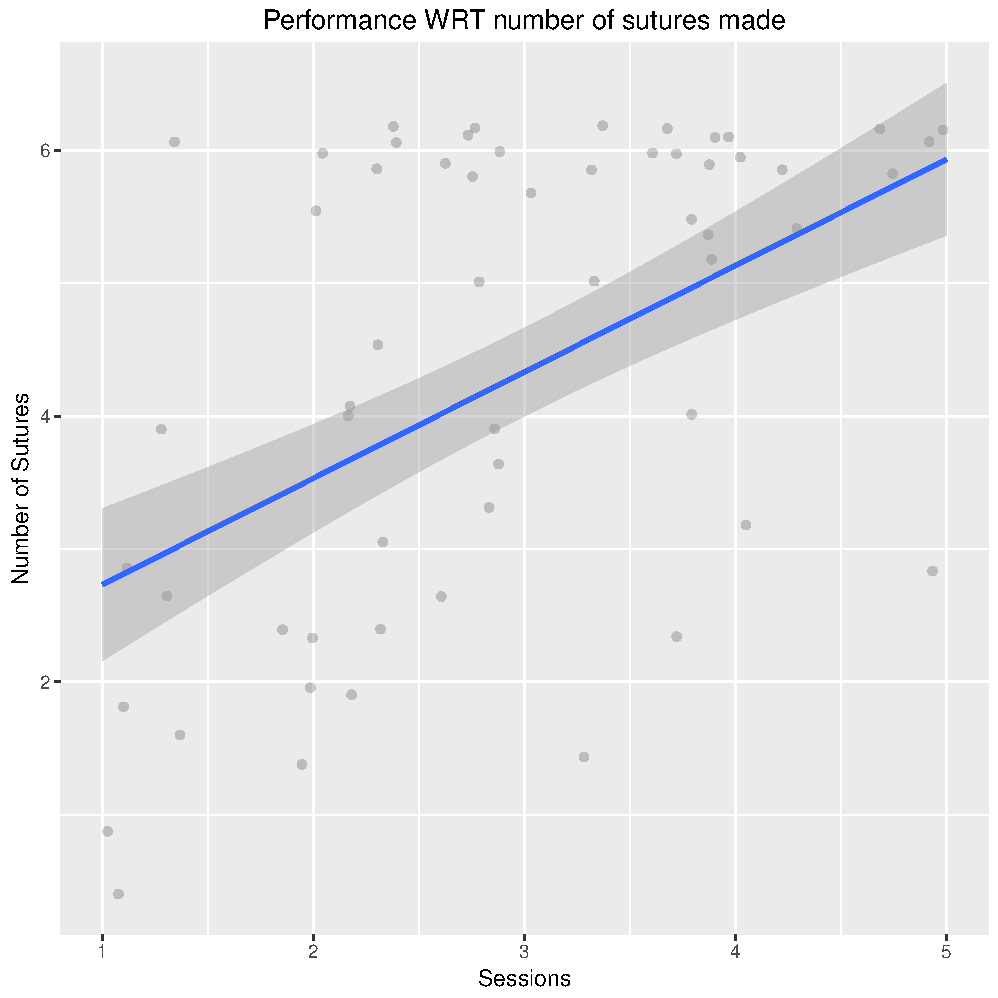
\includegraphics[width=\linewidth]{PerformanceWRTSutures.pdf}
	\end{minipage}
	\hfill
	\begin{minipage}[c]{0.45\linewidth}
	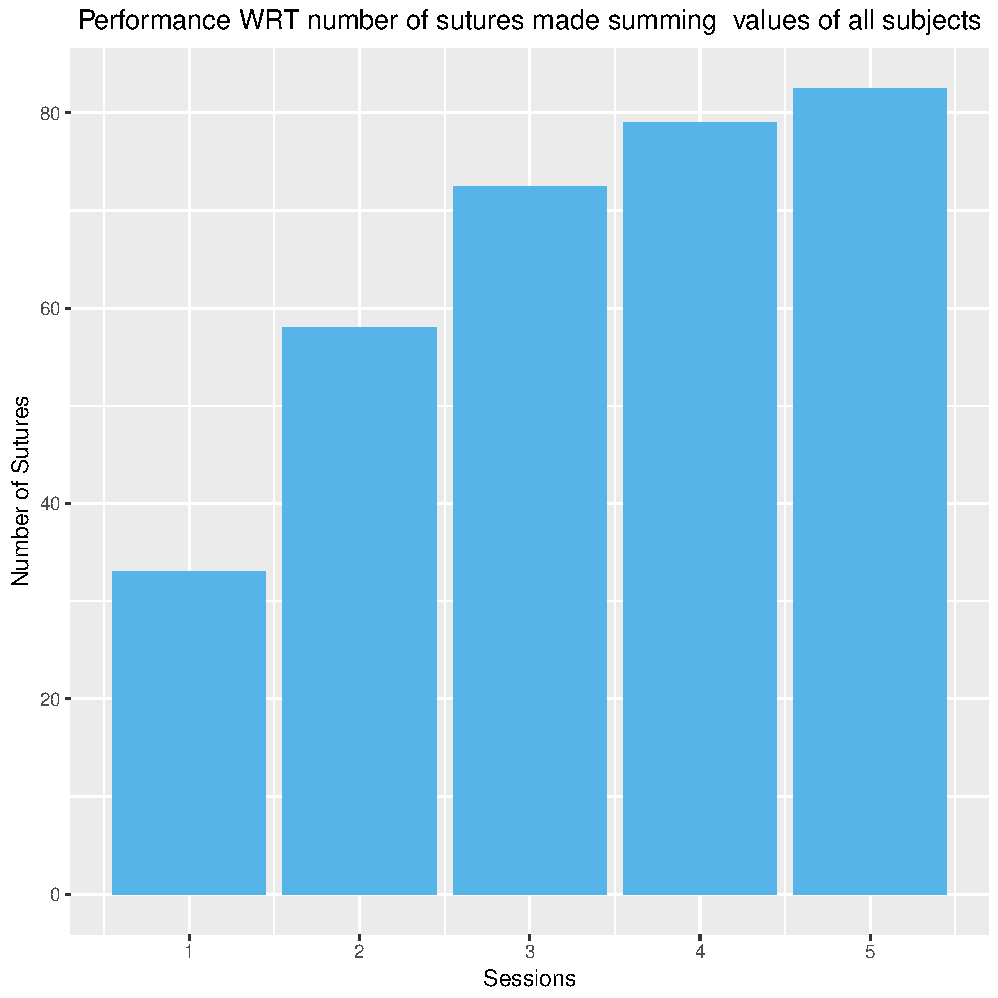
\includegraphics[width=\linewidth]{PerformanceWRTSutures_bar.pdf}
	\end{minipage}
\end{figure}
 \end{frame}
 \begin{frame}{Linear Model}{ Performance Analysis of Suturing Task Contd.}
\begin{itemize}
  \item {The number of sutures increase with decrease in time across session.}
   \item {This indicates the better performance of the subjects with increase in sessions.}
      \end{itemize}\begin{figure}
	\centering
	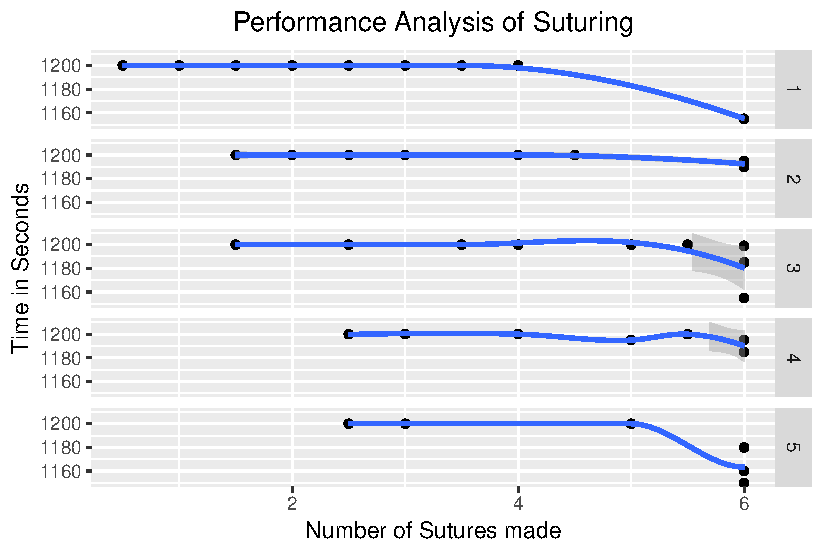
\includegraphics[width=0.5\textwidth]{SuturingVsTime.pdf}
	\centering
\end{figure}
 \end{frame}
 
 \begin{frame}{Hypothesis Testing}{Analysis of Scorers on Task}
\begin{itemize}
  \item {There is effect of Scorer on Suturing not Cutting}
      \end{itemize}
\begin{figure}[!htb]
	\begin{minipage}[c]{0.45\linewidth}
	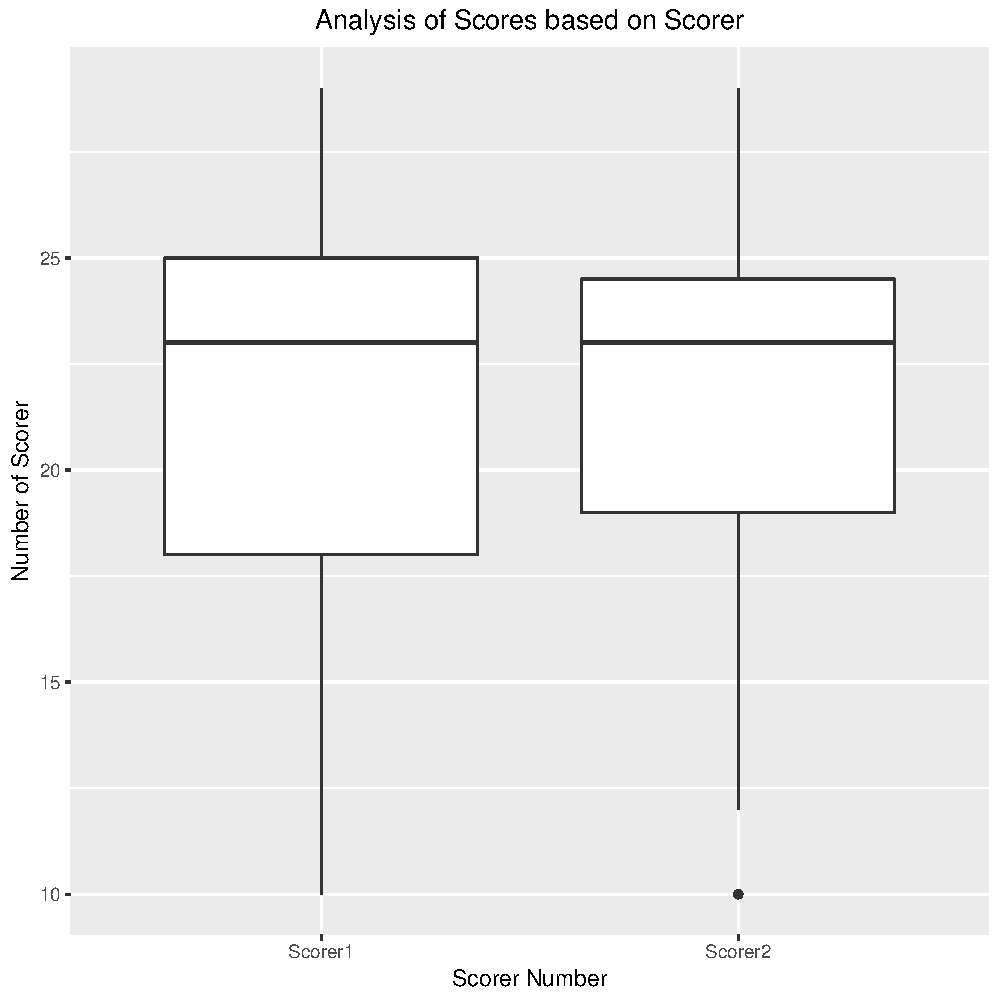
\includegraphics[width=\linewidth]{Cutting_ScorerVsScore.pdf}
	\caption{Cutting Task}
	\end{minipage}
	\hfill
	\begin{minipage}[c]{0.45\linewidth}
	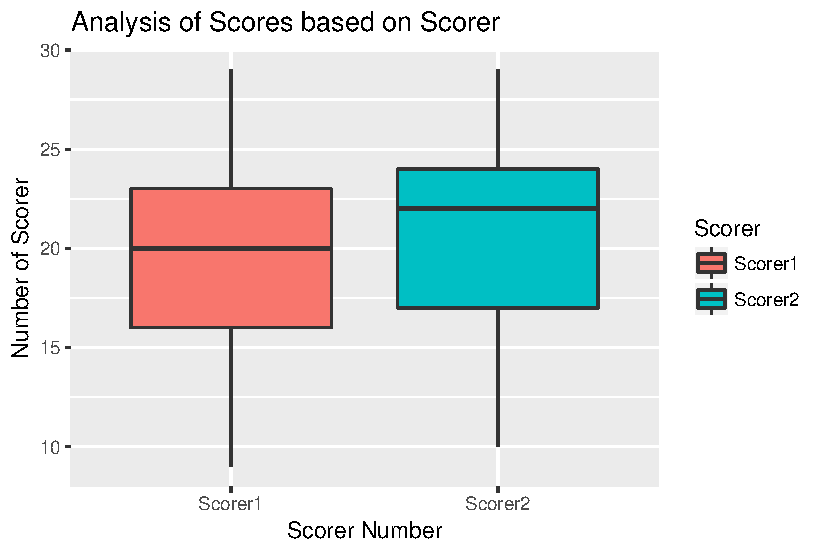
\includegraphics[width=\linewidth]{Suturing_ScorerVsScore.pdf}
	\caption{Suturing Task}
	\end{minipage}
\end{figure}
 \end{frame}
 
 
 







\section{Second Main Section}

\subsection{Another Subsection}

\begin{frame}{Blocks}
\begin{block}{Block Title}
You can also highlight sections of your presentation in a block, with it's own title
\end{block}
\begin{theorem}
There are separate environments for theorems, examples, definitions and proofs.
\end{theorem}
\begin{example}
Here is an example of an example block.
\end{example}
\end{frame}

% Placing a * after \section means it will not show in the
% outline or table of contents.
\section*{Summary}

\begin{frame}{Summary}
  \begin{itemize}
  \item
    The \alert{first main message} of your talk in one or two lines.
  \item
    The \alert{second main message} of your talk in one or two lines.
  \item
    Perhaps a \alert{third message}, but not more than that.
  \end{itemize}
  
  \begin{itemize}
  \item
    Outlook
    \begin{itemize}
    \item
      Something you haven't solved.
    \item
      Something else you haven't solved.
    \end{itemize}
  \end{itemize}
\end{frame}



% All of the following is optional and typically not needed. 
\appendix
\section<presentation>*{\appendixname}
\subsection<presentation>*{For Further Reading}

\begin{frame}[allowframebreaks]
  \frametitle<presentation>{For Further Reading}
    
  \begin{thebibliography}{10}
    
  \beamertemplatebookbibitems
  % Start with overview books.

  \bibitem{Author1990}
    A.~Author.
    \newblock {\em Handbook of Everything}.
    \newblock Some Press, 1990.
 
    
  \beamertemplatearticlebibitems
  % Followed by interesting articles. Keep the list short. 

  \bibitem{Someone2000}
    S.~Someone.
    \newblock On this and that.
    \newblock {\em Journal of This and That}, 2(1):50--100,
    2000.
  \end{thebibliography}
\end{frame}

\end{document}


